\documentclass[10pt]{beamer}

\usepackage{amsfonts}
\usepackage{subfiles}
\usepackage[T2A]{fontenc}
\usepackage[utf8]{inputenc}
\usepackage[russian]{babel}

\usepackage{amsmath, amsfonts, amssymb, amsthm, mathtools, mathrsfs}
\usepackage{wasysym, dsfont}
\usepackage{graphicx}
\usepackage{float}
\usepackage{wrapfig}

\usepackage{caption}
\usepackage{subcaption}
\usepackage{longtable}
% \usepackage{subfigure}

\usepackage{multicol}
\DeclareMathOperator*{\argmax}{\arg\!\max}
\DeclareMathOperator*{\argmin}{\arg\!\min}

\mode<presentation>
{
	\usetheme{boxes}
	\beamertemplatenavigationsymbolsempty
	
	\setbeamertemplate{footline}[page number]
	\setbeamersize{text margin left=1.5em, text margin right=2.0em}
}
\newcommand\blfootnote[1]{%
	\begingroup
	\renewcommand\thefootnote{}\footnote{#1}%
	\addtocounter{footnote}{-1}%
	\endgroup
}
\newcommand\FontUP{\fontsize{12}{12}\selectfont}


\title[]{Обучение взаимосвязанных информативных представлений в задаче генерации образов}
\author{Охотников Никита Владимирович}
\institute{МФТИ}
\date{2023-2024}


\begin{document}

\begin{frame}
  \titlepage
\end{frame}


\begin{frame}
	\frametitle{Введение}
	\begin{block}{Цель}
		\begin{itemize}
			\item Исследовать проблемы дополнения, генерации и оценки образов, состоящих из элементов заранее заданного конечного множества
		\end{itemize}
	\end{block}	
	\vfill
	\begin{block}{Проблемы}
		\begin{itemize}
			\item Высокая дисперсия оценки образа и сложность построения объективных критериев
			\item Нетривиальная взаимосвязь элементов образа 
			\item Практическая невозможность решения полным перебором задач к нему сводящихся
		\end{itemize}
	\end{block}	
	\vfill
	\begin{block}{Необходимо}
		\begin{itemize}
			\item Изучить возможности аппроксимации точного решения, в случае когда оно существует, но невычислимо
			\item Рассмотреть способы моделирования связей между частями внутренней структуры образов
		\end{itemize}
	\end{block}	
\end{frame}


\begin{frame}
	\frametitle{Постановка задачи}
		\begin{block}{Основные понятия и обозначения}
			\begin{itemize}
				\item Основная единица данных, рассматривающаяся в работе -- элемент одежды, далее будем называть его \textit{объектом} или \textit{элементом}, множество всех рассматриваемых объектов -- $\mathcal{X}$
				
				\item Каждый объект $X\in\mathcal{X}$ есть пара $X = (I, T)$ из соответственно изображения о текстового описания.  $\mathcal{I}$ -- множество изображений объектов.
				
				\item Для каждого элемента $X$ определена \textit{категория} $C_x$, из множества категорий $\mathcal{C}$, а множество всех элементов разбивается на подмножества $\mathcal{X}_{C_i}$элементов с общей категорией.
				
				\item 	Некоторое подмножество $O = \{X_i\}_{i=1}^k\subset \mathcal{X}$ множества всех элементов будем называть \textit{образом}, если
				\begin{enumerate}
					\item $O\neq\{\O\}$
					\item $|O| \leqslant K$
					\item $\forall X_i, X_j \in O, i\neq j\longrightarrow C_{X_i} \neq C_{X_j}$
				\end{enumerate}
				где $K$ -- определяемая задачей константа. 
				Множество всех образов $\mathcal{O}$.
				Из такого определения следует, в частности:
				$$O\in\mathcal{O}, O'\subset O \longrightarrow O'\in\mathcal{O}$$
			\end{itemize}
		\end{block}					
\end{frame}

\begin{frame}
	\frametitle{Постановка задачи}
	\begin{block}{Основные понятия и обозначения}
		\begin{itemize}
			\item Для элементов и образов будем рассматривать \textit{функции близости}
			$$S_X:~\mathcal{X}\times \mathcal{X}\longrightarrow [-1,1], ~~\forall X\in\mathcal{X}~S_X(X,X) = 1$$
			$$S_O:~\mathcal{O}\times \mathcal{O}\longrightarrow [-1,1], ~~\forall O\in\mathcal{O}~S_O(O,O) = 1$$
			Такой функцией может выступать например косинусное сходство в некотором латентном пространстве.
			
			\item Для оценки образов введем функцию \textit{оценки} или \textit{совместимости} его элементов: 
			$$\mathcal{S}:~2^\mathcal{X}\longrightarrow [0,1]$$
			причем выполнено следующее:
			$$\forall O \in \mathcal{O}:~\mathcal{S}(O) > 0$$
			$$\forall O' \in 2^\mathcal{X} \setminus \mathcal{O}: \mathcal{S}(O') =0$$
			\textit{Совместимостью} или \textit{оценкой совместимости} образа $O$ будем называть результат применения функции совместимости к этому образу $\mathcal{S}(O)$
		\end{itemize}
	\end{block}					
\end{frame}


\begin{frame}
	\frametitle{Постановка задачи}
	\begin{block}{Оценка образа}
		Задача оценки образа -- это классическая задача регрессии направленная на получения аппроксимации функции оценки $ \mathcal{S}$: \\
		\begin{itemize}
			\item \textbf{Дано:}\\
			$\{O_1\dots O_n\}\subset \mathcal{O}$\\
			$\{\mathcal{S}(O_1)\dots\mathcal{S}(O_n)\}$
			\item \textbf{Требуется:}\\
			Найти наилучшую в некотором смысле аппроксимацию функции $\mathcal{S}$ функциями заданного класса, т.е. решить задачу оптимизации:\\
			$$\hat{\mathcal{S}}= \argmin_{S\in\mathscr{S}}\left[\frac{1}{N} \sum\limits_{i=1}^N\mathcal{L}(\mathcal{S}(O_i), S(O_i))\right]$$
			где $\mathcal{L}(\cdot, \cdot)$ некоторая метрика, например евклидова, а $\mathscr{S}$ -- рассматриваемое множество функций, например нейросети заданной архитектуры.
		\end{itemize}
\end{block}					
\end{frame}


\begin{frame}
	\frametitle{Постановка задачи}
	\begin{block}{Описание образа}
		Задача описания образа есть задача построения наилучшего текстового описания для данного образа по изображениям его элементов. Полагая функцию оценки известной получаем:\\
		\begin{itemize}
			\item \textbf{Дано:}\\
			$\{X_i\} = O_n, ~|O_n| = n$ --- образ, где $X_i = (I_i, \O),~I_i\in\mathcal{I},~i=\overline{1, n}$ --- его элементы с пустым текстовым описанием. \\
			$O_n(T) = \{X_i(T) = (I_i, T)\}_{i=1}^n$ для некоторого общего описания $T$\\
			\item \textbf{Требуется:}\\
			Найти оценку $\hat{T}$ общего для всех элементов описания $T$, максимизирующую значение функции оценки $\mathcal{S}(O_n)$, т.е.: \\
			$$\hat{T}= \argmax_{T}\mathcal{S}(O_n(T))$$
		\end{itemize}
		В данном случае задача генеративная --- лучшее описание находится, из решения задачи максимизации функции оценки, а не просто выбирается из заранее заданного конечного множества.
	\end{block}					
\end{frame}


\begin{frame}
	\frametitle{Постановка задачи}
	\begin{block}{Дополнение (восстановление) образа}
		Задача дополнения образа -- есть задача выбора в некотором смысле наилучшего набора элементов из $\mathcal{X}$ для дополнения данного образа:
		\begin{itemize}
			\item \textbf{Дано:}\\
			$O_n\in\mathcal{O}, ~|O| = n$ \\
			$k \in \mathbb{N}, ~k> n$ --- количество недостающих элементов\\
			$J\subset\mathbb{N},~|J| = m\geqslant k$ --- индексы категорий недостающих элементов\\
			$\{\hat{T_i}\}_{i=1}^k$ --- текстовые представления недостающих элементов, возможно пустые. В случае если предлагается только текстовое описание всего образа $T$, рассматривается $\forall i \in \overline{1,k}: ~T_i = T$.
			
			\item \textbf{Требуется:}\\
			Найти наилучшее в смысле максимизации функции оценки дополнение образа $O_n$ до $O_k\in\mathcal{O}, |O_k|=k$ элементами из категорий $\{C_j\}_{j\in J}$, т.е. решить следующую задачу:
		\end{itemize}
	\end{block}					
\end{frame}


\begin{frame}
	\frametitle{Постановка задачи}
	\begin{block}{Дополнение (восстановление) образа}
		$$\{\hat{X_i}\}_{i=1}^k= \argmax_{\{X_i\}_{i=1}^k\in\bigcup\limits_{j\in J}\mathcal{X}_{C_j}} \bigg{[}\alpha \cdot \mathcal{S}\left(O_n\cup\{X_i\}_{i=1}^k\right) + $$
		
		$$+ (1-\alpha) \cdot \sum\limits_{i=1}^k S_X((I_i, T_i), (I_i, \hat{T_i}))\cdot\mathbb{I}\{\hat{T_i}\neq\O\}  \bigg{]}$$				
		здесь $X_i = (I_i, T_i)$, $\alpha\in[0,1]$. Второе слагаемое отвечает за соответствие предсказанного элемента предъявленному текстовому представлению и равно нулю, если представление пусто. Задача, в отличие от предыдущей, дискриминативная и  может быть решена точно полным перебором всех объектов из $\mathcal{X}$.
	\end{block}					
\end{frame}


\begin{frame}
	\frametitle{Постановка задачи}
	Задача генерации состоит в выборе образа произвольного размера, наиболее подходящего к предоставленному текстовому описанию. В терминах введенных выше получаем:
	
	\begin{itemize}
		\item \textbf{Дано:}\\
		$T$ --- текстовое описание образа.
		
		\item \textbf{Требуется:}\\
		Найти наилучший в смысле максимизации функции оценки образ $O\in\mathcal{O}$ элементы которого наилучшим образом соответствуют предложенному описанию $T$, т.е.:
		$$ \hat{O} = \argmax_{k,O = \{X_i\}_{i=1}^{k},  O\in\mathcal{O}} \left[\alpha \cdot \mathcal{S}(O) + (1-\alpha) \cdot \sum\limits_{i=1}^{k} S_X((I_i, T_i), (I_i, T))\cdot\mathbb{I}\{\hat{T}\neq\O\}  \right]$$				
		здесь $X_i = (I_i, T_i)$, $\alpha\in[0,1]$. 
		Стоит заметить, что если зафиксировать $k=1$, получаем обычную задачу поиска наиболее подходящего под описание элемента в коллекции. Учитывая то, что множество образов определено множеством элементов и определением образа, задача генерации образа также является дискриминативной и состоит в переборе всех возможных образов.
	\end{itemize}			
\end{frame}


\begin{frame}
	\frametitle{Теоретическая часть}
	\begin{itemize}
		\item Элементы равнозначны и задачи симметричны к перестановке $\Longrightarrow$ разумно рассматривать операции эквивариантные относительно группы перестановок.
	
		\item Опустим вопрос выбора способа получения латентных представлений элементов образа и будем использовать
		 полученные с помощью предобученной модели
				
	 	\item В качестве функции оценки возьмем модель из статьи\footnote{\url{https://doi.org/10.48550/arXiv.2204.04812}}.
		
		 \item Рассмотрим задачу дополнения образа. В случае пустого описания недостающих элементов без заранее определенных категорий, с учетом формальной постановки получаем задачу:
		   \begin{itemize}
		   	\item \textbf{Дано:}\\
		   	$O_n\in\mathcal{O}, ~|O| = n$ --- исходный образ \\
		   	$k \in \mathbb{N}, ~k > n$ --- количество недостающих элементов\\					
		   	\item \textbf{Задача:}\\
		   	$$\{\hat{X_i}\}_{i=1}^k= \argmax_{\{X_i\}_{i=1}^k\subset\mathcal{X}} \mathcal{S}\left(O_n\cup\{X_i\}_{i=1}^k\right)$$
		   \end{itemize}
	   \end{itemize}
\end{frame}


\begin{frame}
	\frametitle{Дополнение образа}
	\begin{block}{Дискретный подход}
		\begin{itemize}
			\item Один из подходов к задаче -- приближенный перебор. 
			\item В таком случае, можно рассмотреть полный граф на вершинах $\mathcal{X}\setminus O_n \cup \{X_{init}\}$, где $X_{init}$ -- дополнительная начальная вершина. \\
			Тогда задача эквивалентна максимизации \textit{оценки} пути $X_{init}, X_1, X_2\dots X_k$ в таком графе. Где под \textit{оценкой} пути понимается оценка образа $O_n\cup\{X_1\dots X_k\}$
			\item Жадные бейзлайны:
			\begin{itemize}
				\item $X_1 = \argmax\limits_{X\in\mathcal{X}}{\mathcal{S}(O_n\cup X)},~\dots , X_k = \argmax\limits_{X\in\mathcal{X}\setminus \bigcup\limits_{i=1}^{k-1} X_i} \mathcal{S}(O_n\cup X)$
				\item $X_1 = \argmax\limits_{X\in\mathcal{X}}{\mathcal{S}(O_n\cup X)},~\dots , X_k = \argmax\limits_{X\in\mathcal{X}\setminus \bigcup\limits_{i=1}^{k-1} X_i} \mathcal{S}(O_n\cup X_1\dots X_{k-1}\cup X)$
			\end{itemize}
			\item Предложение: использовать алгоритм beam-search, активно применяемый в языковых моделях. Beam-search в граничных случаях вырождается либо в полный перебор, либо во второй из двух жадных алгоритмов выше.
		\end{itemize}
	\end{block}
\end{frame}


\begin{frame}
	\frametitle{Дополнение образа}
	\begin{block}{Непрерывный подход}
		\begin{itemize}
			\item Задача дополнения --- задача дискретной оптимизации. Однако:
				\begin{itemize}
					\item Фукнция оценки по постановке непрерывна по всем элементам и дифференцируема почти всюду (задана нейросетью)
					\item Есть доступ не только к значению функции оценки, но и градиенту по любому параметру в любой точке
				\end{itemize}
			\item Идея: заменим дискретную задачу непрерывной следующего вида:
			 	$$\{\hat{X_i}\}_{i=1}^k= \argmax_{\{X_i\}_{i=1}^k\subset\mathbb{R}^d} \mathcal{S}\left(O_n\cup\{X_i\}_{i=1}^k\right)$$
			 \item Полученная задача разрешима за разумное время какой либо модификацией стохастического градиентного спуска
			 \item При некоторых ограничениях на функции активации функция оценки к тому же липшицева
			 \item Таким образом, в случае довольно богатой доступной коллекции $\mathcal{X}$ стоит ожидать, что выбор 
			 $X_i = \argmin\limits_{X\in\mathcal{X}}\rho(X, \hat{X_i}),~i=\overline{1,k},$
			 где $\rho$ -- некоторая мера близости между $X$ и $\hat{X_i}$, позволит получить хорошее приближенное решение исходной задачи
		\end{itemize}
	\end{block}
\end{frame}


\begin{frame}
	\frametitle{Базовый эксперимент}
	\begin{block}{Жадные алгоритмы}
		\begin{itemize}
			\item Датасет Polyvore, 17000 образов из 65000 объектов
			\item Рассмотрим небольшое подмножество
			\item Считаем распределение оценок исходных образов
			\item Из каждого образа случайным образом удаляем 2 элемента 
			\item Рассматриваем дополнение получившихся образов 2-мя элементами жадным перебором			
		\end{itemize}
	\end{block}
\end{frame}


\begin{frame}
	\frametitle{Базовый эксперимент}
	\begin{block}{Жадные алгоритмы}
		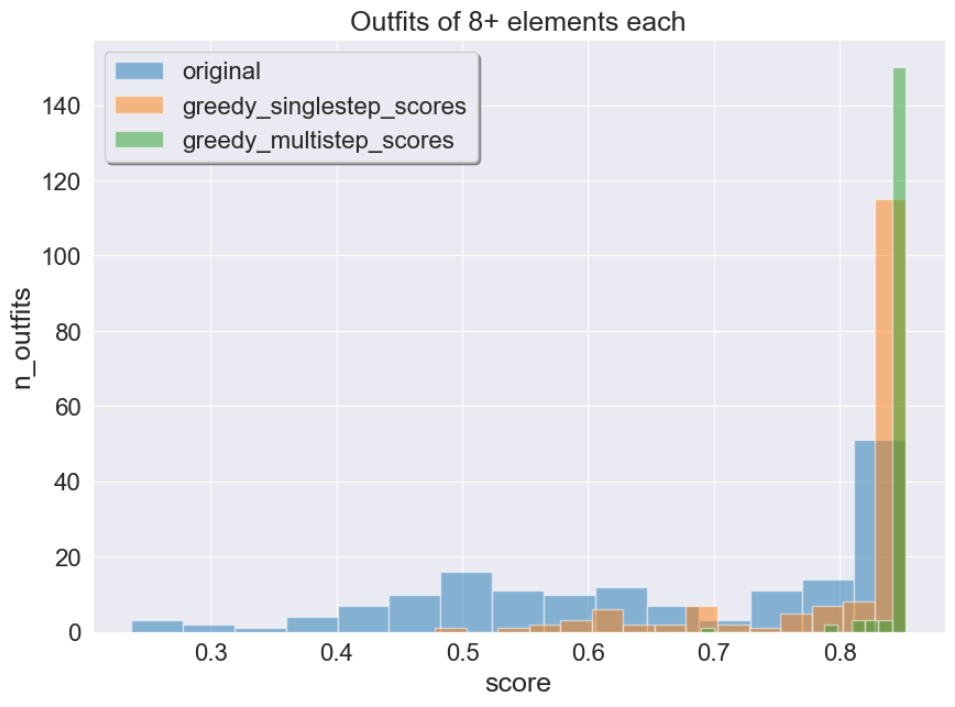
\includegraphics[scale = 0.52]{figures/greedy_at_least_8.png}
	\end{block}
\end{frame}


\begin{frame}
	\frametitle{Базовый эксперимент}
	\begin{block}{Жадные алгоритмы}
		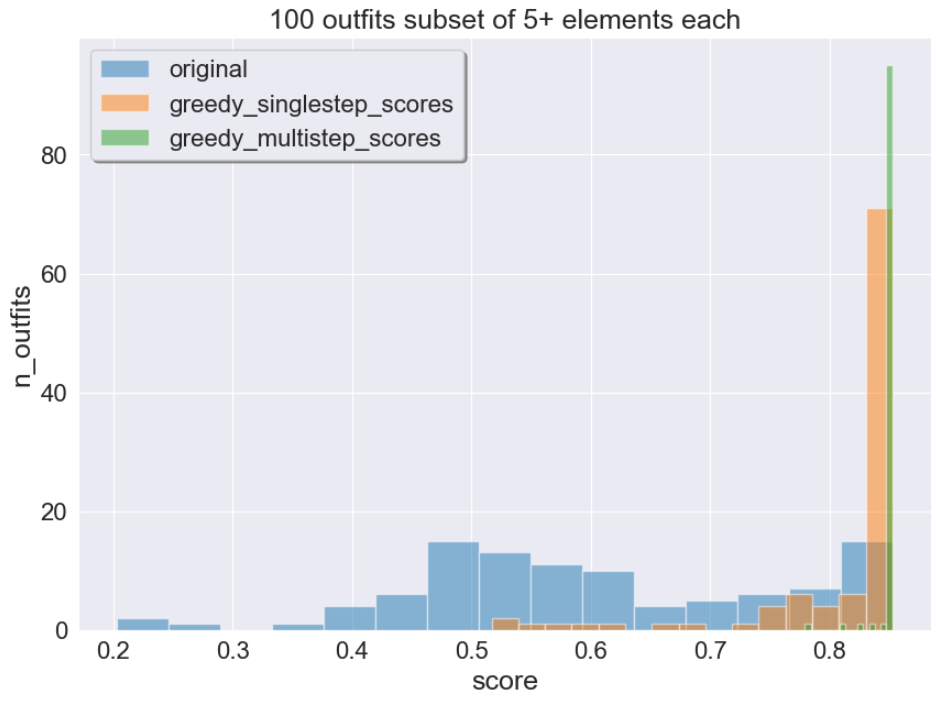
\includegraphics[scale = 0.52]{figures/greedy_at_least_5_subset100.png}
	\end{block}
\end{frame}


\begin{frame}
	\frametitle{Базовый эксперимент}
	\begin{block}{Непрерывная аппроксимация}
		\begin{itemize}
			\item Рассматриваем те же самые образы, удаляем из каждого 2 элемента и рассматриваем дополнение получившихся образов
			\item Замораживаем веса модели оценки
			\item Добавляем 2 обучаемых эмбединга для недостающих элементов
			\item С помощью оптимизатора Adam получаем эмбединги, максимизирующие оценку
			\item Выбираем из всей коллекции элементы, ближайшие к полученным по некоторой метрике, в данном случае взяты $L_1, L_2, L_{10}$
			\item Вычисляем оценку получившегося образа
		\end{itemize}
	\end{block}
\end{frame}

\begin{frame}
	\frametitle{Базовый эксперимент}
	\begin{block}{Непрерывная аппроксимация}
		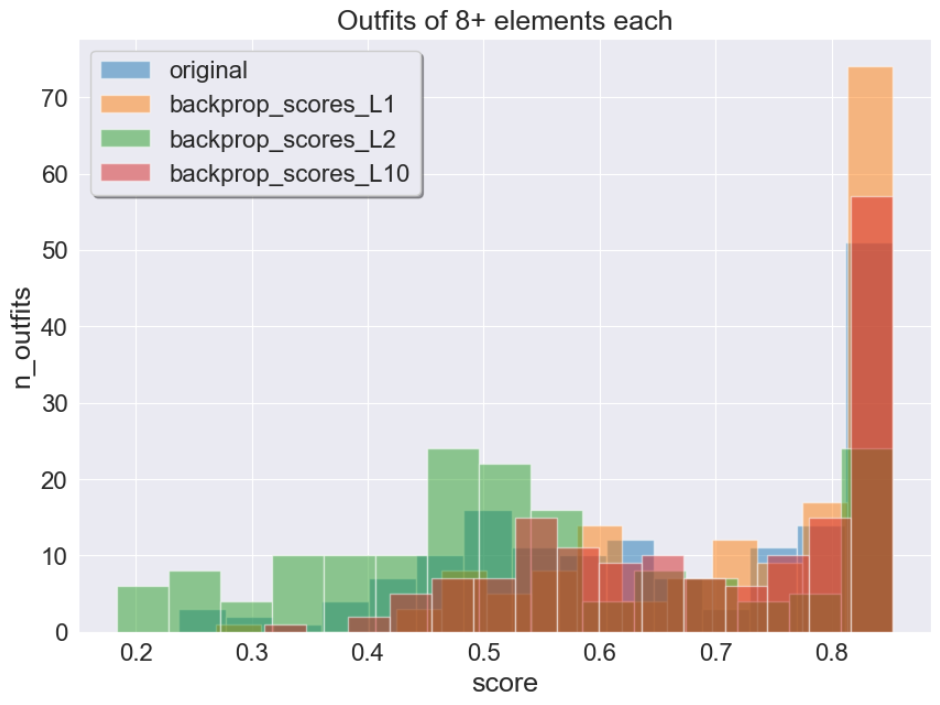
\includegraphics[scale = 0.52]{figures/backprop_at_least_8.png}
	\end{block}
\end{frame}

\begin{frame}
	\frametitle{Базовый эксперимент}
	\begin{block}{Непрерывная аппроксимация}
		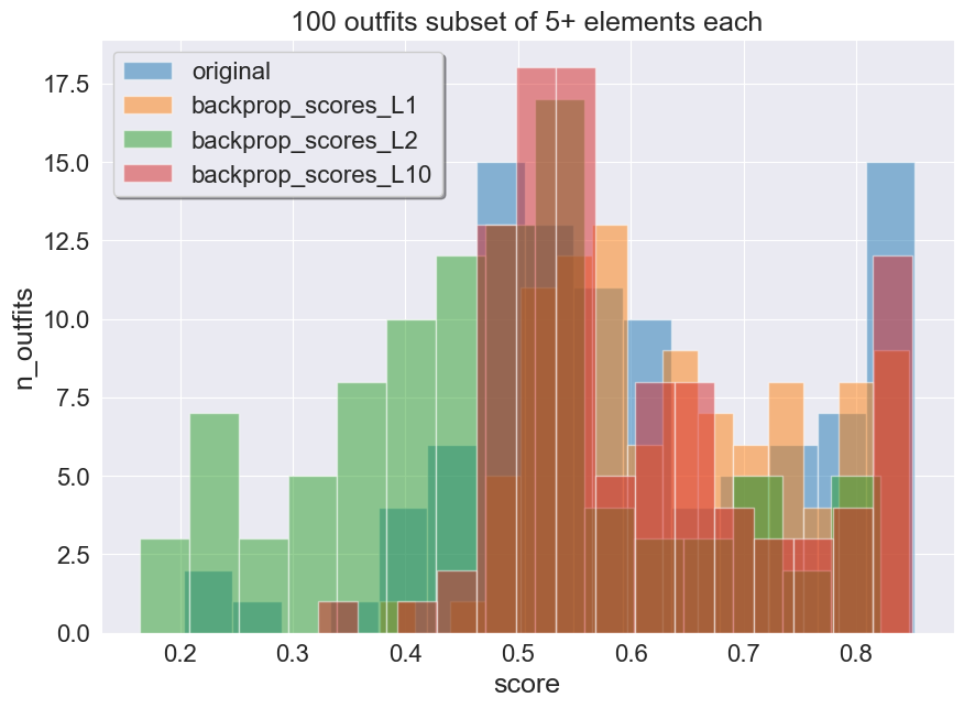
\includegraphics[scale = 0.52]{figures/backprop_at_least_5_subset100.png}
	\end{block}
\end{frame}

\begin{frame}
	\frametitle{Базовый эксперимент}
	\begin{block}{Сравнение}
		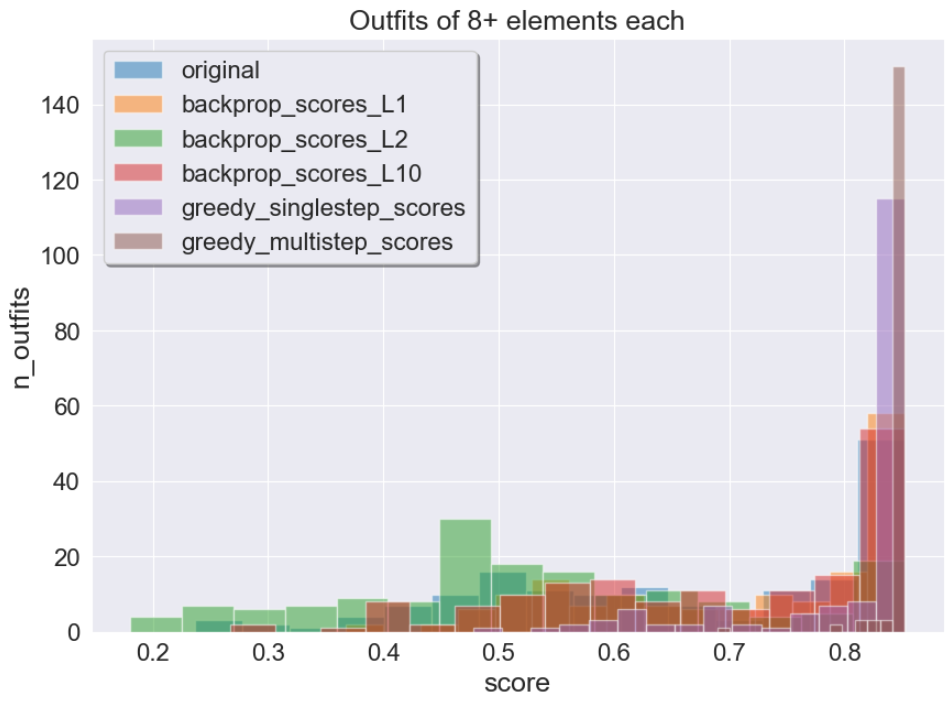
\includegraphics[scale = 0.52]{figures/greedy_and_backprop_at_least_8.png}
	\end{block}
\end{frame}

\begin{frame}
	\frametitle{Базовый эксперимент}
	\begin{block}{Сравнение}
		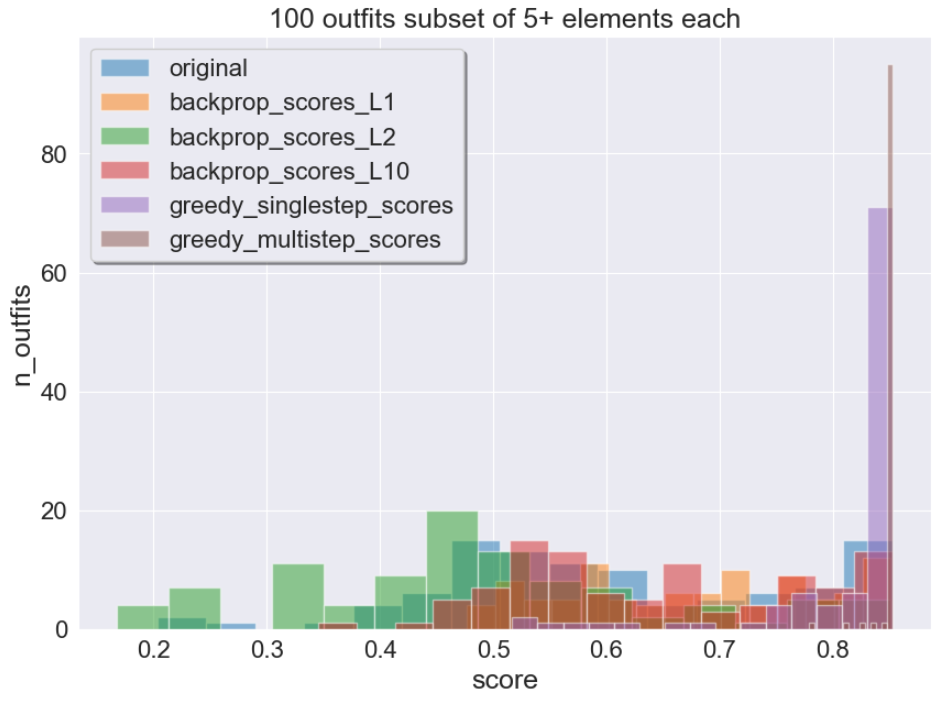
\includegraphics[scale = 0.52]{figures/greedy_and_backprop_at_least_5_subset100.png}
	\end{block}
\end{frame}


\begin{frame}
	\frametitle{Базовый эксперимент}
	\begin{block}{Выводы}
		\begin{itemize}
			\item Жадные алгоритмы показывают хороший результат, но вычисления крайне не эффективны и занимают слишком много времени
			\item Метод непрерывного восстановления векторных представлений недостающих элементов серьезно уступает жадным
			\item Структура пространства представлений элементов слишком сложна, чтобы простые метрики близости позволяли выбрать лучший элемент коллекции 
			\item Предлагается рассмотреть возможности агрегации представлений всех элементов перед выбором ближайшего для учета структуры пространства и взаимодействия элементов между собой.
			\item Агрегация может быть обучаемой. С учетом симметрии задачи, предлагается рассмотреть графовую нейронную сеть
			\item Исходя из постановки задачи, необходимо рассмотреть способы поощрения инвариантности к порядку выбора элементов
			\item Для обучения в дальнейшем можно применять элементы выбранные жадным образом, поскольку более точное решение задачи вряд ли достижимо за разумное время.
				
		\end{itemize}
	\end{block}
\end{frame}




\end{document}
